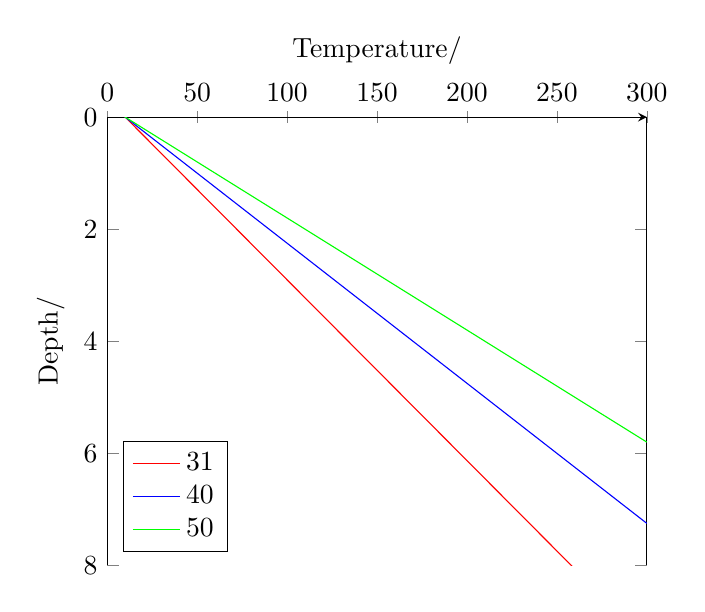
\begin{tikzpicture}
    \begin{axis}[y dir = {reverse},
                 xlabel = {Temperature/\unit{\degreeCelsius}},
                 ylabel = {Depth/\unit{\km}},
                 xmin = 0,
                 xmax = 300,
                 ymin = 0,
                 ymax = 8,
                 axis x line=top,
                 legend style={at={(0.03,0.03)}, anchor=south west},]
        \addplot[color=red,domain=0:300]{(x-10)/31};
        \addlegendentry{\qty{31}{\degreeCelsius\per\km}}
        \addplot[color=blue,domain=0:300]{(x-10)/40};
        \addlegendentry{\qty{40}{\degreeCelsius\per\km}}
        \addplot[color=green,domain=0:300]{(x-10)/50};
        \addlegendentry{\qty{50}{\degreeCelsius\per\km}}
    \end{axis}
\end{tikzpicture}